% #############################################################################
% This is Chapter 4
% !TEX root = ../main.tex
% #############################################################################
% Change the Name of the Chapter i the following line
\fancychapter{Architecture}
\cleardoublepage
% The following line allows to ref this chapter
\label{chap:arch}

The objective of the system was to develop a device in a box format to enable users to establish safe channels of communication. This is achieved with a safe and secure device which is personal to each individual. In order to secure the communications between users, the device saves the user's sensitive data, such as keys, and performs all security critical operations.
The system is designed so that each user has it's own physical box.

% -----------------------------------------------------
% -----------------------------------------------------
\section{Components}\label{chap:arch:components}

\begin{figure}[h]
    \centering
    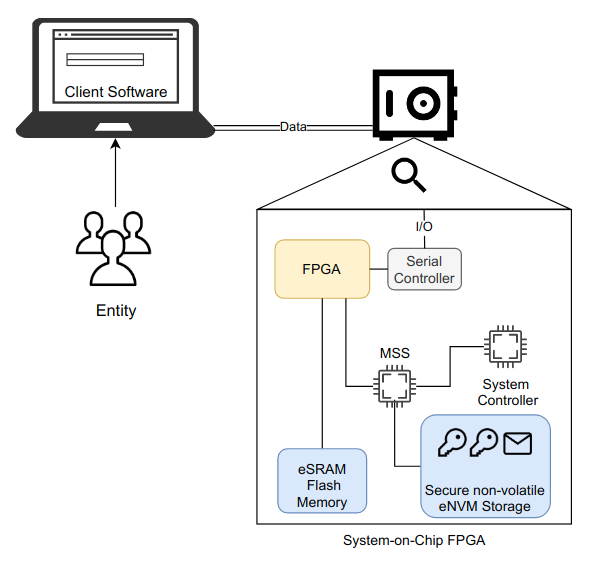
\includegraphics[width=0.7\textwidth]{./Images/main-components.png}
    \caption{System Components}
    \label{fig:components}
\end{figure}

The system architecture, depicted in figure~\ref{fig:components}, is composed of two main components: the physical box which responsible for securing the data, and the client software on the user's computer, which communicates with the box.
The client software sends and receives data through the device's serial I/O port, which exposes an \ac{API} to access its operations.
With this connection the entity can signal the device to perform the desired operations, through the client software.
The device integrates a \ac{FPGA}, \ac{MSS}, secure eNVM storage and flash memory for configuration. The \ac{MSS} has an embedded ARM processor, connected to the system controller which provides several cryptographic services. The secure eNVM allows storage of keys, data and secure boot code.
The \ac{MSS} uses the keys stored in the eNVM, with the cryptographic algorithms in the system controller.

% -----------------------------------------------------
% -----------------------------------------------------
\section{Operations}\label{chap:arch:ops}

The system operations will ensure the system requirements and services are fulfilled.
For the user to be able to execute them, he first must authenticate himself to the device. This is done with a \ac{PIN} or password, which identifies the user. Once authenticated, the operations will be available to the user to be executed in the box.

The operations are split in three types:
\begin{itemize}
    \item Administration operations configure authentication and communication parameters;
    \item The data exchange operations provide the cryptographic services to secure communications;
    \item Communication management operations manage the keys used to secure connections.
\end{itemize}

% -----------------------------------------------------
\subsection{Administration Operations}\label{chap:arch:ops:administration}

The administration operations will allow the user to manage the authentication related parameters.
The only operations of this type is to change the authentication \ac{PIN}. The device will be initialized from fabric with a default \ac{PIN} which must be supplied to the user. Before performing any operation the user should change his PIN to begin secure communications.

% The administrator authenticates himself to the device, begins the registration process and allows the user to insert their name and \ac{PIN}.
% -----------------------------------------------------
\subsection{Data Exchange Operations}\label{chap:arch:ops:data}

The main operations will be responsible to secure the communications between users. These operations will fulfill the confidentiality, authentication and non-repudiation services.

% When a user wishes to generate a signature for a piece of data, he must send the data indicating he wishes a qualified signature. The device will compute and return the signature for the user to use.
\begin{itemize}
    \item Secure data exchange with confidentiality and authentication. The objective of this operation is to send and receive data to and from the device. Plaintext data will be returned to the user encrypted and authenticated with their key stored inside the device. In the case of encrypted and authenticated messages, an error will be returned if the decryption was unsuccessful, otherwise, the user will receive the plaintext data;
    \item Digital Signature operation will provide non-repudiation to a piece of data. The user will send the information to the box, and the subsequent signature will be returned, which can be used to verify the data's authorship. To verify a signature, the user sends it to the device, and receives either success or failure to verify.
\end{itemize}

% -----------------------------------------------------
\subsection{Communication Management Operations}\label{chap:arch:ops:key}

These operations will handle key exchange when new keys need to be generated and exchanged between users, to enable further communications, and to import other user's public keys. This will serve the secure storage and key management services.

The first operations will enable the user to ask for a new key, generated inside the box, in order to securely send it to another user. The user receiving the new key, generated by another user, will receive and store the key inside the box.
The final operation will provide a way to import other user's public keys, as well as export their personal public key, to be shared with another user.

% This also opens the possibility for the symmetric keys to have an expiration date, to avoid overuse, and reduce the possibility of being compromised. When they expire, new ones can be exchanged.
% -----------------------------------------------------
% -----------------------------------------------------

% --- authentication ----
\subsection{Authentication}\label{chap:problem:services:auth}
Every user must authenticate himself, before using the device. This is done by providing a \ac{PIN}, which the device will verify before unlocking the session for the user.

The device will come from fabric with a default authentication \ac{PIN}. This number can be changed by the users.

For personal devices, there is only the owner, but for groups and entities, there can be multiple users. In this case, there are two different ways to authenticate. The simplest is not to authenticate the person using the device, but have a single authentication \ac{PIN} for the entity. All the user's with permission to communicate in behalf of the entity, must know the \ac{PIN}.

The second option, is to authenticate the user itself. The advantage of this approach is there can be a log of which users used the device and when, and what messages were sent and received for each user.
This would entail a more complex process where, each user allowed to use the device, must register with a name and individual \ac{PIN} code. The initial \ac{PIN} code, would be used as an administration code, which allows registering users, and accessing the logs of user operations and message transactions.

It is worth nothing only the users are authenticated, the device does not authenticate itself to the user.

% -----------------------------------------------------
\subsection{Initial State}\label{chap:problem:scenarios:init}

The users will receive the device with a pair of asymmetric keys, a private and public, generated inside the device from fabric.
Each device will have the user's public keys, whom he wishes to communicate.
The user can request whose public keys he wants, before the device is initialized in fabric.
This allows the users to share symmetric keys between them, which they can user to begin trading data securely.
The device can also come with the symmetric keys already shared and stored in each user device.

% -----------------------------------------------------
\subsection{Communications}\label{chap:problem:services:comms}
In order to secure communications, the following services must be guaranteed: confidentiality, integrity and authentication.
The system must also give an option to provide non-repudiation to documents or files, by means of digital signatures.

% -----------------------------------------------------
\subsection{Key management}\label{chap:problem:services:key}
The device must store all the symmetric and asymmetric keys related to the entity or individual who owns the device.

The device must support secure storage in order to store the user's sensitive information, such as the cryptographic keys used for communication.
Additionally, the device should have physical tamper-resistant measures and mechanisms in place, in case of an intrusion, such as, permanent erasure of all sensitive data. 
This means that even if an attacker is in possession of the physical device, it should be extremely difficult or even impossible to extract any information from it.

These keys must never be exposed to the outside environment of the device to ensure the security of communications and independence of the system.

All cryptographic operations must also be performed inside the device.

Key management operations should be supported, namely: symmetric key generation, symmetric key revocation, if communications are suspected to be compromised, and importation of other user's public keys.

Each entity has one pair of asymmetric keys, stored in their device, a private and a public.

For each channel of communication between individual users, groups or entities, the same symmetric key is stored in both devices.

When a new user wants to establish secure communications with an existing user or a group, he must share his public key with the user, ideally physically to ensure no one is impersonated. After this they can securely share symmetric keys, and establish a new secure communication channel when the keys are stored in their devices.

The users will receive the device with a pair of asymmetric keys, a private and public, generated inside the device from fabric. Each device will have the user's public keys, whom he wishes to communicate. The user can request whose public keys he wants, before the device is initialized in fabric. This allows the users to share symmetric keys between them, which they can user to begin trading data securely. The device can also come with the symmetric keys already shared and stored in each user device.

\subsubsection{Device Standardization}

The solution should work with a plethora of devices, which will increase the adoptability of the solution among clients. This entails the use of a widely established protocol, which clearly defines a set of functions and standards the system should follow.
This is where the \ac{PKCS} \#11 standard is again relevant. It allows operations to be standardized across different devices, increasing the range of supported devices. By implementing the system in accordance with these guidelines, it will have a higher device interoperability.
